\documentclass[a4paper, 12pt]{article}

\usepackage{cmap}					
\usepackage{mathtext} 		% русские буквы в формулах		
\usepackage[T2A]{fontenc}			
\usepackage[utf8]{inputenc}			
\usepackage[english,russian]{babel}

\usepackage{amsmath,amsfonts,amssymb,amsthm,mathtools}
\usepackage{icomma} % 'умная' запятая

\mathtoolsset{showonlyrefs=true} % Показывать номера только у тех формул, на которые есть \eqref{} в тексте.

\usepackage{euscript}
\usepackage{mathrsfs}
\usepackage{etoolbox}
\usepackage{ upgreek }


\usepackage{hyperref}
\usepackage[usenames,dvipsnames,svgnames,table,rgb]{xcolor}
\hypersetup{				% Гиперссылки
	unicode=true,           % русские буквы в раздела PDF\\
	pdfstartview=FitH,
	pdftitle={Заголовок},   % Заголовок
	pdfauthor={Автор},      % Автор
	pdfsubject={Тема},      % Тема
	pdfcreator={Создатель}, % Создатель
	pdfproducer={Производитель}, % Производитель
	pdfkeywords={keyword1} {key2} {key3}, % Ключевые слова
	colorlinks=true,       	% false: ссылки в рамках; true: цветные ссылки
	linkcolor=blue,          % внутренние ссылки
	citecolor=green,        % на библиографию
	filecolor=magenta,      % на файлы
	urlcolor=NavyBlue,           % на URL
}

%%% Страница 
\usepackage{extsizes} % Возможность сделать 14-й шрифт
\usepackage{geometry}  
\geometry{left=20mm,right=20mm,top=25mm,bottom=30mm} % задание полей текста

\usepackage{titleps}      % колонтитулы
\newpagestyle{main}{
	\setheadrule{.4pt}                      
	\sethead{}{}{}
	\setfootrule{.4pt}                       
	\setfoot{}{}{ \thepage} 
}      
\pagestyle{main}  

%%%  Текст
\setlength\parindent{1.25cm}         % Устанавливает длину красной строки 0pt
\sloppy                                        % строго соблюдать границы текста
\linespread{1.3}                           % коэффициент межстрочного интервала
\setlength{\parskip}{0.5em}                % вертик. интервал между абзацами
%\setcounter{secnumdepth}{0}                % отключение нумерации разделов
%\setcounter{section}{-1}         % Чтобы сделать нумерацию лекций с нуля
\usepackage{multicol}				          % Для текста в нескольких колонках
%\usepackage{soul}
\usepackage{soulutf8} % Модификаторы начертания

%% Перенос знаков в формулах 
\newcommand*{\hm}[1]{#1\nobreak\discretionary{}
{\hbox{$\mathsurround=0pt #1$}}{}}

\usepackage{graphicx}  
\graphicspath{{images/}{images2/}}  % папки с файлами
\setlength\fboxsep{3pt} % Отступ рамки \fbox{} от рисунка
\setlength\fboxrule{1pt} % Толщина линий рамки \fbox{}
\usepackage{wrapfig} 
\usepackage{caption} % Создание пустых заголовков

%% Работа с таблицами
\usepackage{array,tabularx,tabulary,booktabs} 
\usepackage{longtable}
\usepackage{multirow}

%% Новые функции
\DeclareMathOperator{\sgn}{\mathop{sgn}}
\DeclareMathOperator{\M}{\mathop{mod}}
\DeclareMathOperator{\cont}{\mathop{cont}}
\DeclareMathOperator{\scl}{\mathop{scl}}

\newcommand{\tit}[1]{%
\textit{#1}%
}

\newcommand{\tbf}[1]{%
\textbf{#1}%
}

\newcommand{\wt}[1]{%
\widetilde{ #1 }%
}

\newcommand{\pair}[2]{%
(#1, #2)%
}

\newcommand{\abs}[1]{%
\left| #1 \right|%
}

\newcommand{\av}[1]{%
\left \langle #1 \right \rangle%
}

\newcommand{\rev}[1]{%
\frac{1}{#1}%
}

\newcommand{\wpart}[1]{%
\left \lfloor #1 \right \rfloor%
}

\newcommand{\br}[1]{%
\left( #1 \right)%
}

\newcommand{\sqrbr}[1]{%
\left[ #1 \right]%
}

\newcommand{\figbr}[1]{%
\left\{ #1 \right\}%
}

\newcommand{\eqmod}[3]{%
#1 \equiv #2 ~ \M ~ #3%
}

\newcommand{\FT}[1]{%
\mathcal{F} \sqrbr{#1}%
}

\newcommand{\EXTFT}[3]{%
\mathcal{F}_{ #2 \to #3 } \sqrbr{#1}%
}

\newcommand{\IFT}[1]{%
\mathcal{F}^{-1} \sqrbr{#1}%
}

\newcommand{\EXTIFT}[3]{%
\mathcal{F}_{ #2 \to #3 }^{-1} \sqrbr{#1}%
}

\newcommand{\LT}[1]{%
\mathcal{L} \sqrbr{#1}%
}

\newcommand{\EXTLT}[3]{%
\mathcal{L}_{ #2 \to #3 } \sqrbr{#1}%
}

\newcommand{\ILT}[1]{%
\mathcal{L}^{-1} \sqrbr{#1}%
}

\newcommand{\EXTILT}[3]{%
\mathcal{L}_{ #2 \to #3 }^{-1} \sqrbr{#1}%
}

\newcommand{\domdef}[1]{%
\mathscr{D} \br{#1}%
}

\newcommand{\scal }[2]{%
\br{#1 \cdot #2 }%
}

\newcommand{\norm}[1]{%
\| #1 \|%
}

\newcommand{\topologconv}[1]{%
{\stackrel {#1 }{\longrightarrow }}
}



%% Сокращения команд
\def\RR{\mathbb{R}}
\def\QQ{\mathbb{Q}}
\def\ZZ{\mathbb{Z}}
\def\NN{\mathbb{N}}
\def\FF{\mathbb{F}}
\def\CC{\mathbb{C}}
\def\Zp{\mathbb{N}_0}
\def\Tau{\mathcal{T}}

\let\Rar\Rightarrow
\let\rar\rightarrow
\let\LRar\Leftrightarrow
\let\hkar\hookrightarrow
\let\drar\dashrightarrow
\let\conv\longrightarrow
\let\weakconv\rightharpoondown

\let\inf\infty

\let\degree\circ

\let\lor\vee
\let\land\wedge

\let\leq\leqslant  
\let\geq\geqslant

\let\eps\varepsilon
\let\al\upalpha
\let\phi\varphi
\let\Om\Omega
\let\om\omega
\let\lam\lambda
\let\Lam\Lambda
\let\Th\Theta
\let\th\theta
\let\De\Delta
\let\ga\gamma
\let\Ga\Gamma  
\let\XOR\oplus

% Сокращенния в тексте
\newcommand{\BFS}{\ensuremath{BFS~}}
\newcommand{\DFS}{\ensuremath{DFS~}}
\newcommand{\beginproof}{\noindent \tbf{Доказательство:} }
\newcommand{\conclude}{\noindent \tbf{Вывод:} }

\newcounter{counterprop}
\setcounter{counterprop}{0}

\newcounter{counterdef}
\setcounter{counterdef}{0}

\newcounter{countertheorem}
\setcounter{countertheorem}{0}

%% быстрое оформление
\theoremstyle{plain} % стиль по умолчанию
\newtheorem{theorem}[countertheorem]{Theorem}
\newtheorem{proposition}[counterprop]{proposition}
\newtheorem{lemma}{Лемма}[section]

 
\theoremstyle{definition} % "Определение"
\newtheorem{corollary}{Следствие}
\newtheorem*{problem}{Problem}
\newtheorem{defenition}[counterdef]{defenition}
 
\theoremstyle{remark} % "Примечание"
\newtheorem*{remark}{Замечание}
\newtheorem*{example}{Пример}


\begin{document}
\begin{problem} \tit{(Sylvester's problem)} \\
Let $ a_1, a_2,  \dots , a_m $ be the points in $\RR^d$. Given these points we need to find an spheroid, that contains all points with the minimum volume (or equivalently, with the minimum radius )
\end{problem}
\noindent \tbf{Solution:} \\
In other words we need to find solution of the minimization task:
\begin{equation} \label{def: target function}
\phi(x) = \underset{i = \overline{1 , m } }{\max} \br{ \| a_i - x  \|   } \to \min, ~ x \in \RR^d
\end{equation}
Note that $\phi(x)$ is point-wise maximum of $m$ convex function it means that we can use subdifferential calculus for searching the extremum point of $\phi(x)$.

We will use the following theorems from subdifferential  calculus:
\begin{theorem} \label{th: D-M theorem}
\tit{(Dubovitsky - Milutin)}\\
Let $f_i(x), ~ i = \overline{1, n} $ is convex functions $S \to \RR^d$ (where $S$ is open and conves set) and all of these functions are continuous at a point $x_0 \in S $ and $f(x) = \underset{i = \overline{1, n} }{\max} (f_i (x)) $, then
$$
\partial f(x_0) = \mathop{ch} \br{ \bigcup_{j \in I} \partial f_j(x_0)  },
$$  
where $I = \figbr{j : f_j (x_0) = f(x_0)}$ -- set of active indexes,  $\mathop{ch}$ is convex hull.
\end{theorem}
\begin{theorem} \label{th: FL}
\tit{(Fermat Lemma in subdifferential  calculus)}\\
$x_0$ is point of extremum of $f(x)$ if and only if $0 \in \partial f(x_0)$, where $f(x)$ is convex function.
\end{theorem}
\begin{proposition} \label{pr: subdif of norm}
$$
\partial \br{ \| a - x \|} \br{x_0} = \left\{ 
\begin{aligned} 
& B_1(0), \text{ if } x_0 = a \\
& \frac{a-x}{\| a-x \|}, \text{ if } x_0 \neq a
\end{aligned} \right. ,
$$
where $B_1(0) = \figbr{ x \in \RR^d : \| x \| \leq 1 }$\footnote{In general, we we have a case of dual space, but in this article the case of $\RR^d$ with standard metric is considered, so $ \br{\RR^d}^* = \RR^d $} 
\end{proposition}
\begin{proposition} ~\\
Let $\hat{x}$ is a point of extremum $\phi(x)$ (we consider that $m>1$) , then $\abs{I} > 1$ where $I$ is set of active indexes (see theorem \ref{th: D-M theorem})
\end{proposition}
\noindent $\rhd$ \\
Indeed, if $\abs{I} = 1$ (let $I =\figbr{j^*}$) then only $a_{j^*}$ belongs to the boundary of the spheroid, but according to Fermat Lemma (theorem \ref{th: FL} ) and proposition \ref{pr: subdif of norm}  $ x = a_{j^*}$, it means $r=0$ which is not possible in the case of $m>1$. \\
$\lhd$

Let's first consider the case of $\RR^2$. A circle can be defined by two points on the diameter or by three points belonging to it.
If two points belong to a circle, then it is easy to see that the theorem \ref{th: D-M theorem} holds, but we need to check that all other points belong to this circle. Consider three arbitrary points of the set $a_1, a_2, a_3$ (these points do not belong to one line). Let the circle built on them has a center $c$ and the radius $r$. If this circle contains all the other points of the set then we have to check the fulfillment of the theorem \ref{th: D-M theorem}:
$$
0 \in \triangle ABC = \ch \figbr{ \frac{a_i-c}{\| a_i-c \|}, ~ i = 1, 2, 3 }
$$

The following is an algorithm for checking whether a point belongs to a triangle. 
Point $O$ belongs $\triangle ABC$ if and only if $ S_{ABC} = S_{ABO} + S_{ACO} + S_{BCO}$.

\begin{wrapfigure}{r}{0.35 \linewidth}
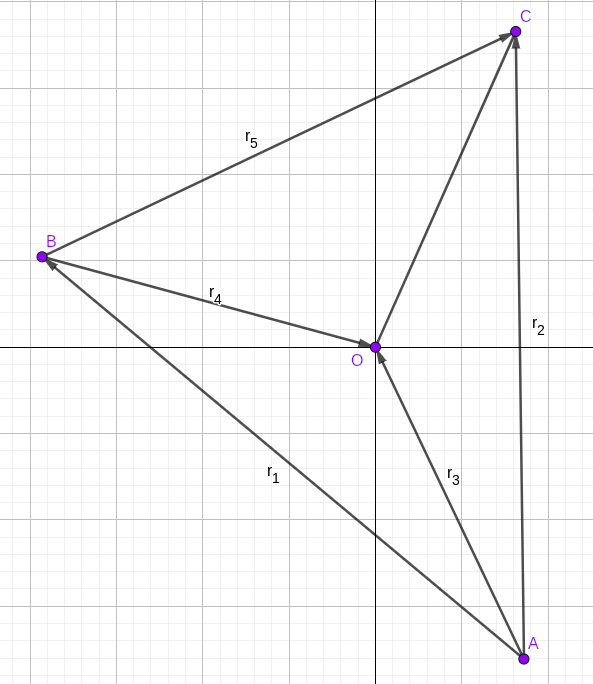
\includegraphics[ width = \linewidth  ]{triangle.png}
\end{wrapfigure}

The square of the triangle can be calculated through the determinant of the matrix formed by the vectors of the sides of the triangle:
$$
S_{ABC} = \frac{1}{2}  \abs{ \det  \begin{pmatrix}
r_1 & r_2
\end{pmatrix} }, ~ S_{ABO} = \frac{1}{2}  \abs{ \det  \begin{pmatrix}
r_1 & r_3
\end{pmatrix} }
$$
the remaining squares can be expressed similarly.

Thus, we present a complete solution algorithm in case $\RR^2$
\begin{enumerate}
\item Iterate through all possible pairs of points. On each such pair, build a circle with a diameter with the ends of these points. If such a circle contains all the other points, then this is the desired circle
\item Iterate through all possible triples of points. Build a circle on each such triple (if these points do not lie on the same straight line).
\begin{enumerate}
\item Check whether the constructed circle contains all points of the set
\item If the previous paragraph is fulfilled, check the fulfillment of the condition of the theorem \ref{th: D-M theorem}
\end{enumerate} 
\end{enumerate}

The presented algorithm is generalized in an understandable way to the case $\RR^d, ~ d > 2$
\end{document}